\documentclass{article}
\usepackage[paper=letterpaper, margin=1in]{geometry}

%% The graphicx package provides the includegraphics command.
\usepackage{graphicx}
%% The amssymb package provides various useful mathematical symbols
\usepackage{amssymb}
%% The amsthm package provides extended theorem environments
%% \usepackage{amsthm}
%% fix strange gensymb error
\usepackage{textcomp}
%% symbols, especially degree
\usepackage{gensymb}
%% scientific units
\usepackage{siunitx}
%% line spacing
\usepackage{setspace}
\doublespacing
%% left justification in tables
\usepackage{array}
\newcolumntype{P}[1]{>{\raggedright\arraybackslash}p{#1}}
%%references
%\usepackage[round]{natbib}
%%landscape orientation
\usepackage{pdflscape}
\usepackage[hyphens]{url}
\usepackage{hyperref}

\graphicspath{ {../data_out/MS_results_revisions/Infection/figures/supplement/} }
\DeclareGraphicsExtensions{.pdf}
\begin{document}

\noindent
\textbf{\LARGE{Spatio-temporal Spillover Risk of Yellow Fever in Brazil}}

\bigskip
\noindent
RajReni B. Kaul, Michelle V. Evans, Courtney C. Murdock, John M. Drake
\smallskip

%\setcounter{tocdepth}{2}
\tableofcontents

\newpage

\section*{Data Collection}

Monthly confirmed cases of yellow fever for each Brazilian Munic\'{i}pio (sub-state administrative units) from 2001 to 2013 were downloaded from the Brazilian government's portal da sa\'{u}de website, \texttt{tabnet} (\url{http://tabnet.datasus.gov.br}) on 05 June 2017.
Confirmed cases were reported by the Ministry of Health Notification of Injury Information System (SINAN-Net) as determined using clinical-epidemiological criteria.

The annual population for each Munic\'{i}pio from 2001 to 2013 was also downloaded from the Brazilian government's portal da sa\'{u}de website,\texttt{tabnet} on 05 June 2017. The estimated population was calculated by the Instituto Brasileiro de Geografia e Estat\'{i}stica (Brazialian Institure of Geography and Statistics) as intercensorial estimates.

Monthly land surface temperature and normalized difference vegetation index (NDVI) data from 2001 through 2013 were downloaded from the NASA Land Processes Distributed Active Archive Center (LPDAAC). The MODIS MOD11C3 product contains monthly temperature data at a 0.05\degree resolution. THE MODIS MOD13A3 product contains monthly NDVI data at a 1 km resolution. Both gridded data products were then aggregated to the municipality level to obtain a monthly spatially averaged temperature and NDVI value for each municipality.

Rainfall data was obtained from the NASA GESDISC data archive in the form of data from the Tropical Rainfall Monitoring Mission from 2001 through 2013. The 3B43 product contains an average rainfall rate for each month at a 0.25\degree resolution. We aggregated the gridded data to the municipality level by taking the spatial mean.

Monthly fire locations were downloaded from the Fire Information for Resource Management System (FIRMS). The MODIS Active Fire Product (MCD14ML) reports fire at a 1 km resolution by month. This data was then aggregated to the total number of fires per municipality by month, and scaled to density by dividing by the municipality's total area.

Primate species richness data was obtained from the IUCN Redlist of Terrestrial Mammals for species in genera known to be susceptible to yellow fever (\textit{Ateles, Aotus, Alouatta, Saimiri, Cebus, Callicebus, Callithrix, Saguinus, Lagothrix}) \cite{bicca-marques2010,hamrick2017}. Individual species' ranges were combined to calculate the number of species found within a municipality, defined as species richness. We also estimated the relative proportion of primate habitat overlapping with agricultural land use per municipality per year. Shapefiles of geographic ranges of each genus were constructed from the above range maps. Yearly land cover data from 2001 - 2013 was downloaded from the NASA Land Processes Distributed Active Archive Center (LPDAAC). The MODIS MCD12Q1 dataset contains yearly land cover categories at a 1 km resolution by year. The proportion of total municipality area that was both agricultural land use and within a genus range was then calculated for each genus.  These proportions were then summed over all nine genera, resulting in a value from 0 - 9 per municipality by year, defined as the Agricultural and Primate Overlap.



\section*{Results}

\subsection*{Summary of YF cases in Brazil}


\begin{figure} [h]
\centering
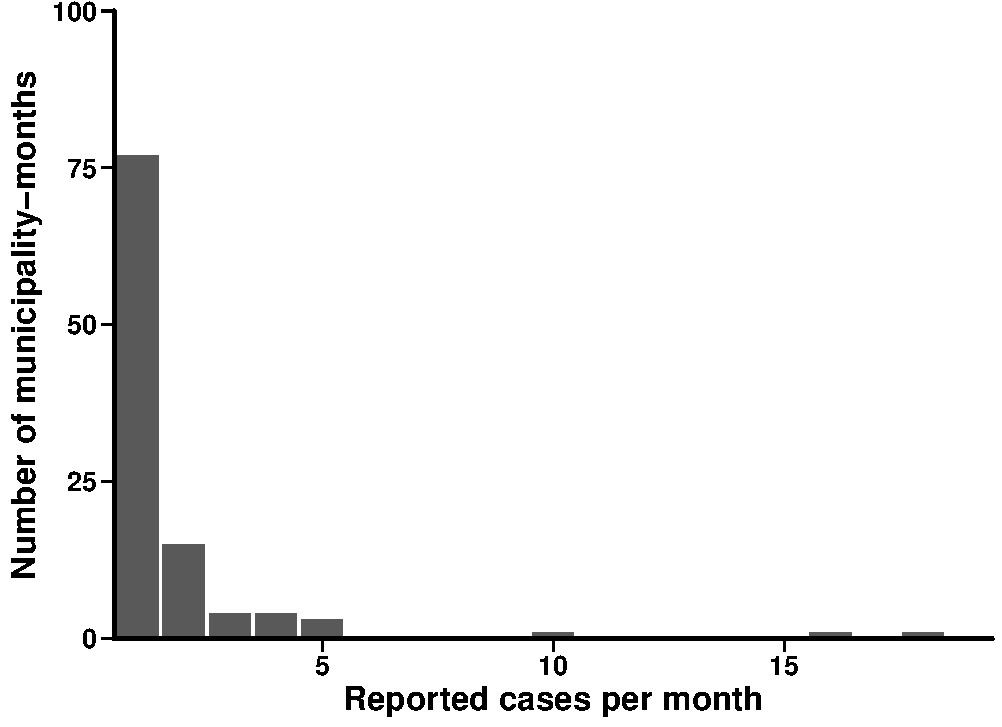
\includegraphics[width=0.5\textwidth]{Hist_Reported_Cases}
\caption{}
\label{}
\end{figure}

\subsection*{Univariate analysis of covariates}




\bibliographystyle{bmc-mathphys} % Style BST file (bmc-mathphys, vancouver, spbasic).
\bibliography{references}

\clearpage

%\begin{table}[h]
%\normalsize
%\centering
%\caption{Data summary. Training and testing dataset used to build the national model, which was then subset into the low reservoir richness (LRR), and high reservoir richness (HRR) regional models. }
%\label{my-label}
%\begin{tabular}{lcclccl}
 %     & \multicolumn{3}{c}{Positive Observations}                          & \multicolumn{3}{c}{Background Observations}                          \\ \cline{2-7}
%Model & \multicolumn{1}{l}{Training} & \multicolumn{1}{l}{Testing} & Total & \multicolumn{1}{l}{Training} & \multicolumn{1}{l}{Testing} & Total   \\ \hline
%National   & 81                           & 35                          & 116   & 607,070                      & 260,174                     & 867,244 \\
%LRR   & 67                           & 28                          & 95    & 584,159                      & 250,346                     & 834,505 \\
%HRR   & 14                           & 7                           & 21    & 22,911                       & 9,828                       & 32,739
%\end{tabular}
%\begin{flushleft}
%\smallskip
%
%\end{flushleft}
%\end{table}

\end{document}
